\documentclass[12pt,oneside]{ctexbook}
\usepackage{amsmath,amsfonts}
\usepackage{amssymb}
\usepackage{rotating}
\usepackage{graphicx}
\newtheorem{definition}[subsection]{定义}
\newtheorem{theorem}[subsection]{定理}
\newtheorem{property}[subsection]{性质}
\newtheorem{method}[subsection]{基本方法}
\newtheorem{problem}[subsection]{典型例题}

%title
\begin{document}
\title{Linear Algebra Knowledge Points Collection}
\author{\kaishu 俞奕成}
\date{\kaishu \today}

\maketitle

Introduction: This article aims to arrage the knowledge points of the Linear Algebra Course for learners in order to improve their understanding and boost the efficiency.
%contents
\setcounter{tocdepth}{2}
\tableofcontents

\newpage

\part{矩阵}

\chapter{矩阵基本概念}
\[\mathbf{A}=(a_{ij})_{m\times n}=
\begin{pmatrix}
    a_{11}&a_{12}&\dots&a_{1n}
    \\a_{21}&a_{22}&\dots&a_{2n}
    \\ \vdots &\vdots &\vdots &\vdots
    \\a_{m1}&a_{m2}&\dots&a_{mn}
\end{pmatrix}\]
A为m行n列的矩阵,\(a_{ij}\)为第i行j列的元素

\section{同型矩阵}
\kaishu
矩阵\(A=(a_{ij})_{m\times n}\) \(B=(b_{ij})_{s\times t}\),\\如果\(m=s,n=t\),则矩阵A和B为同型矩阵。
\\直观:形状相同

\section{相等矩阵}
\kaishu
矩阵\(A=(a_{ij})_{m\times n}\) \(B=(b_{ij})_{s\times t}\),\\
若同型,且\(a_{ij}=b_{ij}\), \(i=1,2,\dots ,m\),\(j=1,2,\dots ,n\)
\\则A,B为相等矩阵.
\\直观:形状相同,且每个位置的元素对应相等

\section{主对角线与主对角元}
\begin{description}
    \item[主对角线] \kaishu 在n阶方阵\(\mathbf{A}\)中,从(1,1)位置到(n,n)位置的直线称为方程的主对角线
    \item[主对角元] \kaishu 主对角线上的元素
\end{description}

\section{常用矩阵}
\begin{description}
    \item[零矩阵]{\kaishu 元素全为0的矩阵称为零矩阵,记为\(\mathbf 0_{m\times n}\)或\(\mathbf 0\)}
    \item[行(列)矩阵] {\kaishu 仅有一行(列)的矩阵}
    \item[行(列)向量]{\kaishu 定义同行(列)矩阵} 
    \item[方阵] \kaishu 行数和列数相同的矩阵
    \item[对角矩阵] \kaishu 除了主对角线上的元素外,其他元素都是0的矩阵,简称为对角阵,记为\(\mathbf A = \mathbf{diag}(a_{11},a_{22},\dots ,a_{nn})\)
    \item[单位矩阵] \kaishu 主对角元全为1的对角矩阵。记为\(\mathbf{E}\)或者\(\mathbf{I}\)
    \item[数量矩阵] \kaishu 主对角元全部相等的对角矩阵。记为\( k \mathbf E \)或者\(k\mathbf E_n\)
    \item[上(下)三角矩阵] \kaishu 主对角线下方(上方)的元素全为0的方阵
    \item[对称矩阵] In matrix \(\mathbf{A}=(a_{ij})_n\), \(a_{ij}=a_{ji}\), \(i,j=1,2,\dots ,n\) \newline \kaishu 直观:关于主对角线对称
    \item[反对称矩阵] In matrix \(\mathbf{A}=(a_{ij})_n\), \(a_{ij}=-a_{ji}\), \(i,j=1,2,\dots ,n\) \newline \kaishu 直观:主对角线上下两块对应位置上的元素互为相反数
\end{description}

\chapter{矩阵的运算}
\section{矩阵的线性运算}
\subsection{定义}
\begin{description}
    \item[数乘] 设\(A=(a_{ij})_{m\times n}\),称\((ka_{ij})_{m\times n}\)为矩阵A与数k的数量乘积,简称数乘,记为\(k\mathbf{A}\)
    \item[负矩阵] 特别地,将\((-1)\mathbf{A}\)记为\(-\mathbf{A}\),称为A的负矩阵
    \item[加法] 设矩阵\(\mathbf{A}=(a_{ij})_{m\times n}\)与\(\mathbf{B}=(b_{ij})_{m\times n}\),//称\(m\times n\)矩阵\(\mathbf{C}=(a_{ij}+b_{ij})_{m\times n}\)
    \item[减法] 称\(\mathbf{A}+(\mathbf{-B})\)为矩阵A与B的差,记为\(\mathbf{A}-\mathbf{B}\)
\end{description}

\subsection{性质} 该部分运算性质与数的运算完全相同,不再赘述
\section{矩阵乘法}
\subsection{定义}
设\(\mathbf{A}=(a_{ij})_{m\times n}\),\(\mathbf{B}=(b_{ij})_{n\times s}\),\(\mathbf{C}=(c_{ij})_{m\times s}\),其中
\[c_{ij}=a_{i1}b_{1j}+a_{i2}b_{2j}+\dots +a_{in}b_{nj}=\sum_{k=1}^n a_{ik}b_{kj}\]
\[i=1,2,\dots ,m;j=1,2,\dots,s,\]
称矩阵\(\mathbf{C}\)为矩阵\(\mathbf{A}\)与矩阵\(\mathbf{B}\)的乘积,记为\(\mathbf{C}=\mathbf{A}\mathbf{B}\)
\subsection{性质}
\begin{enumerate}
    \item \(\mathbf{A}_{m\times n}\mathbf{0}_{n\times s}=\mathbf{A}_{m\times s}\)  ,  \(\mathbf{0}_{s\times m}\mathbf{A}_{m\times n}=\mathbf{0}_{s\times n}\)
    \item \(\mathbf{E_m}\mathbf{A}_{m\times n}=\mathbf{A}_{m\times n}\)     ,     \(\mathbf{A}_{m\times n}\mathbf{E_n}=\mathbf{A}_{m\times n}\)
    \item \(\mathbf{A}(\mathbf{B}\mathbf{C})=(\mathbf{A}\mathbf{B})\mathbf{C}\) (乘法结合律)
    \item \((k\mathbf{A})\mathbf{B}=k(\mathbf{A}\mathbf{B})=\mathbf{A}(k\mathbf{B})\)
    \item \(\mathbf{A}(\mathbf{B}+\mathbf{C})=\mathbf{A}\mathbf{B}+\mathbf{A}\mathbf{C}\) (左分配律), \((\mathbf{B}+\mathbf{C})\mathbf{A}=\mathbf{B}\mathbf{A}+\mathbf{C}\mathbf{A}\) (右分配律)
\end{enumerate}

\subsection{可换矩阵}
\begin{definition}
两个矩阵\(\mathbf{A}\),\(\mathbf{B}\),如果\(\mathbf{AB}=\mathbf{BA}\),那么称矩阵\(\mathbf{A}\),\(\mathbf{B}\)相乘可换,简称\(\mathbf{A}\),\(\mathbf{B}\)可换.
\end{definition}
\subsubsection{一些推论}
\begin{enumerate}
    \item 若\(\mathbf{A}\),\(\mathbf{B}\)相乘可换,则\(\mathbf{A}\),\(\mathbf{B}\)必是同阶方阵
    \item 单位矩阵和与之同阶的方阵相乘可换
    \item 数量矩阵和与之同阶的方阵相乘可换
    \item 同阶对角矩阵相乘可换
\end{enumerate}

\section{方阵的幂}
\begin{definition}
    设\(\mathbf{A}\)是n阶方阵,k为正整数,
    \\k个\(\mathbf{A}\)相乘称为\(\mathbf{A}\)的k次幂,记为\(\mathbf{A^k}\),即\(\mathbf{A^k}= \overbrace{\mathbf{A}\cdot \mathbf{A}\cdot \dots \cdot \mathbf{A}}^{k*A} \)
    \\规定\(\mathbf{A^0}=\mathbf{E_n}\)    
\end{definition}
\begin{property}
    设A为方阵,k,l为非负整数,则
    \[A^k \cdot A^l=A^{k+l} , (A^k)^l=A^{kl}\]
\end{property}
\begin{definition}
    \textbf{方阵的多项式}
    \\ 设\(\mathbf{A}\)是方阵,\(\mathbf{E}\)为与\(\mathbf{A}\)同阶的单位矩阵 \\
    称\(f(\mathbf{A})=a_m\mathbf{A}^m+a_m\mathbf{A}^m+ \dots + a_0E\)是由\(f(x)\)决定的方阵\(\mathbf{A}\)的多项式
\end{definition}
\section{矩阵的转置}
\begin{definition}
    设数域F上的矩阵\(\mathbf{A}=(a_{ij})_{m\times n}\),称\(n\times m\)的矩阵
    \[\begin{pmatrix}
        a_{11}&a_{21}&\dots&a_{m1}
        \\a_{12}&a_{22}&\dots&a_{m2}
        \\ \vdots &\vdots &\vdots &\vdots
        \\a_{1n}&a_{2n}&\dots&a_{mn}
    \end{pmatrix}\]
    为矩阵A的转置矩阵,记为\(\mathbf{A}^\mathrm{T}\)
\end{definition}
\begin{property}
    \textbf{转置矩阵的运算性质}\\
    \begin{enumerate}
        \item \((\mathbf{A}^\mathrm{T})^\mathrm{T}=A\)
        \item \((\mathbf{B}+\mathbf{C})^\mathrm{T}=\mathbf{B}^\mathrm{T}+\mathbf{C}^\mathrm{T}\)
        \item \((k\mathbf{A})^\mathrm{T}=k\mathbf{A}^\mathrm{T}\)
        \item \((\mathbf{A}\mathbf{B})^\mathrm{T}=\mathbf{B}^\mathrm{T}\mathbf{A}^\mathrm{T}\)  \((\mathbf{A}_1\mathbf{A}_2\dots \mathbf{A}_m)^\mathrm{T}=\mathbf{A}_m^\mathrm{T}\mathbf{A}_{m-1}^\mathrm{T}\dots \mathbf{A}_2^\mathrm{T}\mathbf{A}_1^\mathrm{T}\)
        \item 若\(\mathbf{A}\)为方阵,则\((\mathbf{A}^m)^\mathrm{T}=(\mathbf{A}^\mathrm{T})^m\),m为正整数
        \item \(\mathbf{A}\)为对称矩阵\(\Leftrightarrow \mathbf{A}^\mathrm{T}=\mathbf{A}\),\(\mathbf{A}\)为反对称矩阵\(\Leftrightarrow \mathbf{A}^\mathrm{T}=-\mathbf{A}\)
    \end{enumerate}
\end{property}

\section{方阵的迹}
\begin{definition}
    设数域F上的方阵\(\mathbf{A}=(a_{ij})_{m\times n}\) ,称\(\sum\limits_{i=1}^n a_{ii}\)为方阵A的迹,记为\(tr(\mathbf{A})\) ,即\(tr(A)=\sum\limits_{i=1}^n a_{ii}\)
\end{definition}
\begin{property}
    \begin{enumerate}
        \item \(tr(\mathbf{A}+\mathbf{B})=tr(\mathbf{A})+tr(\mathbf{B})\)
        \item \(tr(k\mathbf{A})=ktr(\mathbf{A})\)
        \item \(tr(\mathbf{A}\mathbf{B})=tr(\mathbf{B}\mathbf{A})\)
        \item \(tr(\mathbf{A}^\mathrm{T})=tr(\mathbf{A})\)
    \end{enumerate}
\end{property}
\chapter{可逆矩阵}
\section{定义}
\begin{definition}
    设n阶方阵\(\mathbf{A}\),若存在n阶方阵\(\mathbf{B}\),使得\(\mathbf{A}\mathbf{B}=\mathbf{B}\mathbf{A}=\mathbf{E}\),
    则称矩阵\(\mathbf{A}\)可逆,\(\mathbf{B}\)是\(\mathbf{A}\)的逆矩阵,记作\(\mathbf{B}=\mathbf{A}^{-1}\)。如果不存在这样的\(\mathbf{B}\),则称矩阵\(\mathbf{A}\)不可逆。
\end{definition}

\section{方阵可逆的条件}
\begin{theorem}
    如果n阶方阵\(\mathbf{A}\)可逆,则其逆矩阵唯一。
\end{theorem}

\begin{definition}
    设n阶方阵\(\mathbf{A}=(a_{ij})_{n\times n}\),
    \\ \(\mathbf{A}_{ij}\)为元素\(a_{ij}\)的余子式\(i,j=1,2, \dots ,n\),称矩阵
    \[\begin{pmatrix}
        A_{11}&A_{21}&\dots&A_{n1}
        \\A_{12}&A_{22}&\dots&A_{n2}
        \\\vdots&\vdots&&\vdots
        \\A_{1n}&A_{2n}&\dots&A_{nn}
    \end{pmatrix}\]
    为矩阵\(\mathbf{A}\)的伴随矩阵,记为\(\mathbf{A}^{*}\)(即代数余子式转置排列得到的矩阵)
\end{definition}
\begin{theorem}
    设n阶方阵\(\mathbf{A}=(a_{ij})_{n\times n}\),
    则\(\mathbf{A}\mathbf{A}^*=\mathbf{A}^*\mathbf{A}=\rvert \mathbf{A}\rvert\mathbf{E}\)
\end{theorem}
\begin{theorem}
    n阶方阵\(\mathbf{A}\)可逆的充分必要条件为\(\rvert \mathbf{A} \rvert \neq 0\),且此时
    \[\mathbf{A}^{-1}=\frac{1}{\rvert \mathbf{A} \rvert} \mathbf{A}^*\]
    \textbf{推论} 设\(\mathbf{A}\)为n阶方阵,若存在n阶方阵\(\mathbf{B}\),使得\(\mathbf{A}\mathbf{B}=\mathbf{E}\)(或\(\mathbf{B}\mathbf{A}=\mathbf{E}\)),则\(\mathbf{A}\)可逆且\(\mathbf{B}=\mathbf{A}^{-1}\)
\end{theorem}
\section{可逆矩阵的运算性质}
设\(\mathbf{A}\),\(\mathbf{B}\)均为n阶可逆矩阵,k为非零常数,则
\begin{enumerate}
    \item \((\mathbf{A}^{-1})^{-1}=\mathbf{A}\)
    \item \(k\mathbf{A}\)可逆,且\((k\mathbf{A})^{-1}=\dfrac{1}{k}\mathbf{A}^{-1}\)
    \item \(\mathbf{A}\mathbf{B}\)可逆,且\((\mathbf{A}\mathbf{B})^{-1}=\mathbf{B}^{-1}\mathbf{A}^{-1},\\(\mathbf{A}_{1}\mathbf{A}_2\dots \mathbf{A}_m)^{-1}=\mathbf{A}_{m}^{-1}\dots \mathbf{A}_{2}^{-1}\mathbf{A}_{1}^{-1}\)
    \item 若\(\mathbf{A}^m\)可逆,\((\mathbf{A}^{m})^{-1}=(\mathbf{A}^{-1})^{m}\)
    \item 若\(\mathbf{A}^\mathrm{T}\)可逆,\((\mathbf{A}^\mathrm{T})^{-1}=(\mathbf{A}^{-1})^\mathrm{T}\)
    \item \(\rvert \mathbf{A}^{-1}\rvert=\dfrac{1}{\rvert \mathbf{A} \rvert}\)
\end{enumerate}

\section{可逆矩阵求法}
\subsection{初等变换法求逆矩阵}
见第\pageref{reverseMatrix}页第\ref{reverseMatrix}节

\chapter{分块矩阵}
\section{定义}
\begin{definition}
    把矩阵\(\mathbf{A}_{m \times n}\)用若干条横线和竖线,分成若干小矩阵,每个小矩阵称为\(\mathbf{A}\)的一个子块,以这些子块为元素的形式上的矩阵称为\(\mathbf{A}\)称为A的分块矩阵
\end{definition}
\section{分块矩阵的运算方法}
\subsection{加减法}
与矩阵定义相同,但操作的两个矩阵必须同型并且采用相同的分块法(即每一组对应的分块都应该同型)
\subsection{乘法}
\label{dividedMatrixMulti}
\begin{enumerate}
    \item \(\mathbf{A}\)的列分块法必须与\(\mathbf{B}\)的行分块法相同
    \item 操作方法与矩阵乘法类似:\(\mathbf{C}_{ij}=\sum\limits_{k=1}^s \mathbf{A}_{ik}\mathbf{B}_{kj}\)
\end{enumerate}
\subsection{分块矩阵的转置}
设分块矩阵为\(\mathbf{A}=\begin{pmatrix}
    \mathbf{A}_{11}&\mathbf{A}_{12}&\dots&\mathbf{A}_{1t}
    \\\mathbf{A}_{21}&\mathbf{A}_{22}&\dots&\mathbf{A}_{2t}
    \\ \vdots &\vdots &\vdots &\vdots
    \\\mathbf{A}_{s1}&\mathbf{A}_{s2}&\dots&\mathbf{A}_{st}
\end{pmatrix}\)
\\则\(\mathbf{A}^\mathrm{T}=\begin{pmatrix}
    \mathbf{A}^\mathrm{T}_{11}&\mathbf{A}^\mathrm{T}_{21}&\dots&\mathbf{A}^\mathrm{T}_{t1}
    \\\mathbf{A}^\mathrm{T}_{12}&\mathbf{A}^\mathrm{T}_{22}&\dots&\mathbf{A}^\mathrm{T}_{t2}
    \\ \vdots &\vdots &\vdots &\vdots
    \\\mathbf{A}^\mathrm{T}_{1s}&\mathbf{A}^\mathrm{T}_{2s}&\dots&\mathbf{A}^\mathrm{T}_{ts}
\end{pmatrix}\)
\subsection{分块(反)对角矩阵}
形如\[\mathbf{A}=\begin{pmatrix}
    \mathbf{A}_1&
    \\ &\mathbf{A}_2
    \\ &&\ddots
    \\ &&&\mathbf{A}_s
\end{pmatrix}\]
记为\(\mathbf{A}= \mathbf{diag}(\mathbf{A}_{1},\mathbf{A}_{2},\dots ,\mathbf{A}_{s})\)
,称为分块对角矩阵
\\如果\(\mathbf{A}_{i}\)可逆,则\(\mathbf{A}\)可逆,有\[\mathbf{A}^{-1}=\begin{pmatrix}
    \mathbf{A}^{-1}_1&
    \\ &\mathbf{A}^{-1}_2
    \\ &&\ddots
    \\ &&&\mathbf{A}^{-1}_s
\end{pmatrix}\]
形如\[\mathbf{A}=\begin{pmatrix}
    &&&\mathbf{A}_1
    \\ &&\mathbf{A}_2
    \\ &\begin{turn}{80}\(\ddots\)\end{turn}
    \\ \mathbf{A}_s
\end{pmatrix}\]
称为反对角矩阵,
\\如果\(\mathbf{A}_{i}\)可逆,则\(\mathbf{A}\)可逆,有
\[\mathbf{A}^{-1}=\begin{pmatrix}
    &&&\mathbf{A}^{-1}_s
    \\ &&\begin{turn}{80}\(\ddots\)\end{turn}
    \\ &\mathbf{A}^{-1}_2
    \\ \mathbf{A}^{-1}_1
\end{pmatrix}\]


\chapter{矩阵的初等行变换}
\section{初等行(列)变换}
\begin{definition}
    \kaishu 矩阵的下面三种行为,称之为矩阵的初等行变换(行变换):
\begin{enumerate}
    \item 交换矩阵的i,j两行,记为\(r_i \leftrightarrow r_j \)
    \item 矩阵的第i行非零常数k倍,记为\(kr_i\)
    \item 矩阵的第i行的常数k倍加到第j行,记为\(r_j+kr_i\)(顺序不可反)
\end{enumerate}
\end{definition}

\begin{definition}
    \kaishu 矩阵\(\mathbf{A}^\mathrm{T}\)的行变换,称之为矩阵\(\mathbf{A}\)的初等列变换(列变换):
\begin{enumerate}
    \item 交换矩阵的i,j两列,记为\(c_i \leftrightarrow c_j \)
    \item 矩阵的第i列非零常数k倍,记为\(kc_i\)
    \item 矩阵的第i列的常数k倍加到第j列,记为\(c_j+kc_i\)(顺序不可反)
\end{enumerate}
\end{definition}
\section{矩阵相抵}
\begin{definition}
    矩阵\(\mathbf{A}\)经有限次初等变换得到矩阵\(\mathbf{B}\)则称矩阵\(\mathbf{A}\)与矩阵\(\mathbf{B}\)相抵,记为\(\mathbf{A}\cong \mathbf{B}\)
\end{definition}
\begin{property}
    显然,矩阵相抵有以下性质:
    \begin{enumerate}
        \item 反身性:\(\mathbf{A}\cong \mathbf{A}\)
        \item 对称性:若\(\mathbf{A}\cong \mathbf{B}\),则\(\mathbf{B}\cong \mathbf{A}\)
        \item 传递性:\(\mathbf{A}\cong \mathbf{B}\cong \mathbf{C}\),则\(\mathbf{A}\cong \mathbf{C}\)
    \end{enumerate}
\end{property}

\section{阶梯形矩阵}
\begin{definition}
    满足下面两个条件的矩阵称为行阶梯形矩阵,简称阶梯形矩阵:
\begin{enumerate}
    \item 零行(元素全为零的行)排在所有非零行的下方
    \item 每个非零行的第一个(从左至右)非零元(称为主元)的列标号,从上到下,严格递增
\end{enumerate}
\end{definition}
\begin{definition}
    一个阶梯形矩阵若满足下面两条性质,称之为(行)简化阶梯形(或行最简形)矩阵基本概念
\begin{enumerate}
    \item 主元均为1
    \item 主元所在列的其他元素全为零
\end{enumerate}
\end{definition}



\begin{theorem}
    任何一个矩阵都可以经过初等行变换化为阶梯形矩阵或者简化阶梯形矩阵
\end{theorem}

\section{初等矩阵}
\begin{definition}
单位矩阵经过一次初等变换以后得到的矩阵
\begin{enumerate}
    \item \(\mathbf{E}\xrightarrow[r_i\leftrightarrow r_j]{c_i\leftrightarrow c_j}\mathbf{E}(i,j)\)
    \item \(\mathbf{E}\xrightarrow[kr_i]{kc_i}\mathbf{E}(i(k))\)
    \item \(\mathbf{E}\xrightarrow[r_j+kr_i]{c_i+kc_j}\mathbf{E}(i,j(k))\)
\end{enumerate}
\end{definition}

\begin{theorem}
    \textbf{初等矩阵与初等变换的关系:行左列右}
    \\设\(\mathbf{A}\)是一个\(m \times n\),对\(\mathbf{A}\)进行一次初等行变换相当于在\(\mathbf{A}\)的左边乘一个相应类型的m阶初等矩阵;对\(\mathbf{A}\)进行一次初等列变换相当于在\(\mathbf{A}\)的右边乘以一个相应类型的n阶矩阵
    \\ \textbf{推论}
    初等矩阵都是可逆矩阵,且有
    \begin{enumerate}
        \item \(\mathbf{E}(i,j)^{-1}=\mathbf{E}(i,j)\)
        \item \(\mathbf{E}(i(k))^{-1}=\mathbf{E}(i(\dfrac{1}{k}))\)
        \item \(\mathbf{E}(j,i(k))^{-1}=\mathbf{E}(j,i(-k))\)
    \end{enumerate}
\end{theorem}

\begin{theorem}
    对任意的\(m\times n\)矩阵\(\mathbf{A}\),存在一系列m阶初等矩阵\(\mathbf{P}_1,\mathbf{P}_2,\dots,\mathbf{P}_s\)
    \\及n阶初等矩阵\(\mathbf{Q}_1,\mathbf{Q}_2,\dots,\mathbf{Q}_t\)使得
    \[\mathbf{P}_s\dots \mathbf{P}_2\mathbf{P}_1\mathbf{A}\mathbf{Q}_1\mathbf{Q}_2\dots\mathbf{Q}_t
    =\begin{pmatrix}
        \mathbf{E_r}&\mathbf{0}
        \\ \mathbf{0}&\mathbf{0}
    \end{pmatrix}\]
    为标准形,其中\(\mathbf{E_r}\)为r阶单位矩阵,r是\(\mathbf{A}\)的行阶梯形中非零行的行数
\end{theorem}

\section{一些应用和基本方法}
\begin{method}
    \label{reverseMatrix}
    \textbf{求逆矩阵的初等变换法}
    \\构造矩阵:
    \((\mathbf{A}\quad|\quad\mathbf{E})\xrightarrow[]{r}(\mathbf{E}\quad|\quad\mathbf{A}^{-1})\)
\end{method}

\begin{method}
    \textbf{使用初等变换法求解矩阵方程}
    \[\mathbf{A}\mathbf{X}=\mathbf{B} \Rightarrow \mathbf{X}=\mathbf{A}^{-1}\mathbf{B}\]
    \[(\mathbf{A}\quad|\quad\mathbf{B})_{n\times (n+m)}\xrightarrow{r}(\mathbf{E}\quad|\quad\mathbf{A}^{-1}\mathbf{B})\]
    \\similarly
    \[\mathbf{X}\mathbf{A}=\mathbf{B} \Rightarrow \mathbf{X}=\mathbf{B}\mathbf{A}^{-1}\Rightarrow \mathbf{X}^\mathrm{T}=(\mathbf{A}^\mathrm{T})^{-1}\mathbf{B}^\mathrm{T} \]
    \[(\mathbf{A}^\mathrm{T}\quad|\quad\mathbf{B}^\mathrm{T})_{n\times (n+m)}\xrightarrow{r}(\mathbf{E}\quad|\quad(\mathbf{A}^\mathrm{T})^{-1}\mathbf{B}^\mathrm{T})\]
\end{method}

\section{分块矩阵的初等变换与分块初等矩阵}
\begin{definition}
    \textbf{分块初等矩阵}
    均为矩阵的初等变换和初等矩阵定义的扩展
\end{definition}
\begin{definition}
    对分块矩阵作一次初等行(列)变换,相当于用相应的分块初等矩阵左(右)乘此分块矩阵。
    \\ \textbf{注意:要遵循分块矩阵的乘法中对于两个相乘矩阵的分块法的要求}
    \\具体见\pageref{dividedMatrixMulti}页\ref{dividedMatrixMulti}节
\end{definition}


\chapter{矩阵的秩}
\section{定义}
\begin{definition}
    \textbf{子式}
    \\设\(\mathbf{A}\)为\(m \times n\)的矩阵,在\(\mathbf{A}\)中任取k行k列(\(k\leq min\{m,n\}\)),位于这些行列交叉处的元素按原来的相对位置构成的k阶方阵的行列式,称为矩阵\(\mathbf{A}\)的k级(阶)子式
\end{definition}
\begin{definition}
    \textbf{矩阵的秩}
    \\
    设\(\mathbf{A}\)为\(m \times n\)的矩阵,在\(\mathbf{A}\)中若存在一个r阶子式不等于零,而所有的r+1阶子式都等于零(如果存在的话),称r为矩阵的秩,记为\(r\mathbf(A)\)。规定零矩阵的秩为零
\end{definition}

\section{性质}
\begin{property}
    设矩阵\(\mathbf{A}_{m \times n}\),则
    \begin{enumerate}
        \item 矩阵A的秩是唯一的
        \item \(0\leq \mathbf{A} \leq min\{m,n\}\)
        \item 设\(\mathbf{A_1}\)是\(\mathbf{A}\)的一个部分矩阵,则\(r(\mathbf{A_1}) \leq r(\mathbf{A})\)
        \item 若\(\mathbf{A}\)中存在r阶子式不为零,则\(r(\mathbf{A}) \geq r\);若\(\mathbf{A}\)中所有r阶子式全为零,则\(r(\mathbf{A})<r\)
        \item \(r(\mathbf{A}^\mathrm{T})=r(\mathbf{A})\)
        \item \(r(k\mathbf{A})=\begin{cases}
            r(\mathbf{A}),\quad k \neq 0,
            \\0,\quad k=0.
        \end{cases}\)
        \item 阶梯形矩阵的秩等于它的非零行的个数
        \item 可逆矩阵的秩等于它的阶数
    \end{enumerate}
\end{property}

\section{矩阵的秩的不变性}
\begin{theorem}
    初等变换不改变矩阵的秩
\end{theorem}

\section{与标准型和可逆矩阵的关系}
\begin{theorem}
    对任意的\(m\times n\)矩阵\(\mathbf{A}\),存在一系列m阶初等矩阵\(\mathbf{P}_1,\mathbf{P}_2,\dots,\mathbf{P}_s\)
    \\及n阶初等矩阵\(\mathbf{Q}_1,\mathbf{Q}_2,\dots,\mathbf{Q}_t\)使得
    \(\mathbf{P}_s\dots \mathbf{P}_2\mathbf{P}_1\mathbf{A}\)为简化阶梯形矩阵;且
    \[\mathbf{P}_s\dots \mathbf{P}_2\mathbf{P}_1\mathbf{A}\mathbf{Q}_1\mathbf{Q}_2\dots\mathbf{Q}_t
    =\begin{pmatrix}
        \mathbf{E_r}&\mathbf{0}
        \\ \mathbf{0}&\mathbf{0}
    \end{pmatrix}_{m \times n}\]
    为标准形,其中\(r=r(\mathbf{A})\),且标准形唯一。
    \\ \textbf{一系列重要推论}
    \begin{enumerate}
        \item 任意矩阵\(\mathbf{A}_{m \times n}\),存在一系列m阶可逆矩阵\(\mathbf{P}\)和n阶可逆矩阵\(\mathbf{Q}\),使得
        \[ \mathbf{P}\mathbf{A}\mathbf{Q}=\begin{pmatrix}
            \mathbf{E_r}&\mathbf{0}
            \\ \mathbf{0}&\mathbf{0}
        \end{pmatrix}_{m \times n},r=r(\mathbf{A})\]
        \item n阶矩阵\(\mathbf{A}\)可逆的充分必要条件为\(\mathbf{A}\)的标准形为n阶单位矩阵\(\mathbf{E_n}\)
        \item n阶矩阵\(\mathbf{A}\)可逆的充分必要条件为\(\mathbf{A}=\mathbf{P}_1,\mathbf{P}_2,\dots,\mathbf{P}_k\),其中\(\mathbf{P_i}(i=1,2,\dots,k)\)为初等矩阵
        \item 若\(\mathbf{A_n}\)可逆,则\(\mathbf{A}\)可只经过行变换化为单位矩阵.
        \item 矩阵\(\mathbf{A}_{m\times n},\mathbf{P}_m,\mathbf{Q}_n\)分别为m阶和n阶可逆矩阵,则\[r(\mathbf{P}\mathbf{A})=r(\mathbf{A})=r(\mathbf{A}\mathbf{Q})=r(\mathbf{P}\mathbf{A}\mathbf{Q})\]
        \item 矩阵\(\mathbf{A}_{m \times n}\)与\(\mathbf{B}_{m \times n}\)相抵的充分必要条件为
        \\ \(\exists\)可逆矩阵\(\mathbf{P},\mathbf{Q}\),\(s.t. \mathbf{P}\mathbf{A}\mathbf{Q}=\mathbf{B}\)
    \end{enumerate}
    \begin{theorem}
        \textbf{矩阵的秩与线性方程组解的判别}
        \\见第\pageref{equation&r}页第\ref{equation&r}节
    \end{theorem}
\end{theorem}


\part{线性方程组}
\chapter{数域}
\begin{enumerate}
    \item 设\(\mathbf{F}\)为一个数集,如果\(\mathbf{F}\)中任意两个数做某种运算的结果仍属于\(\mathbf{F}\),称数集F对这种运算封闭
    \item 设\(\mathbf{F}\)是包含0和1的数集,若\(\mathbf{F}\)对四则运算封闭,则称\(\mathbf{F}\)为一个数域,记为F
\end{enumerate}
\chapter{线性方程组的基本概念}
\section{线性方程组定义}
形如
\[\begin{cases}
    a_{11}x_1 + a_{12}x_2 + \dots + a_{1n}x_n = b_1\\
    a_{21}x_1 + a_{22}x_2 + \dots + a_{2n}x_n = b_2\\
    \vdots \\
    a_{m1}x_1 + a_{m2}x_2 + \dots + a_{mn}x_n = b_m
\end{cases}
\]
称为一个m个方程n个未知量的线性方程组,简记为\(m \times n\)的线性方程组或线性系统。其中\(a_{ij} \in F, i=1,2,\dots ,m; j=1,2,\dots,  x_1 , x_2 , \dots , x_n\)为未知变量,\(a_{ij}\)表示第i个方程中的第j个未知量\(x_j\)前面的系数,\(b_i\)为第i个方程的常数项。

\section{解集的定义}
若存在一组数 \(c_1,c_2,\dots ,c_n \in F\) 满足方程组的每个方程,\\则称\(x_1=c_1,x_2=c_2,\dots ,x_n=c_n\) 为方程组的一组解或者一个解,记为\((c_1,c_2,\dots ,c_n)\).方程组的全体解所构成的集合称为该方程组的解集。

\section{同解方程组}
如果两个方程组的解集相同,则称这两个方程组为同解方程组或者两个方程组同解。

\chapter{解的判别与求法}
\section{线性方程组的消元法} 直接对方程组进行消元等操作,此处不再赘述
\section{高斯消元法} 线性方程组对应的增广矩阵\(\mathbf {\tilde A}\)通过初等行变换化为一个(简化)阶梯形矩阵,通过(简化)阶梯形矩阵求解线性方程组的方式,称为线性方程组的高斯消元法。
\subsection{定理:解的不变性} 线性方程组的高斯消元法得到的新方程组与原方程组同解
\subsection{定理:线性方程组解的判别} \(m \times n\)的线性方程组,其增广矩阵化为阶梯形矩阵有r个非零行,期中对应于方程组的系数矩阵部分有s个非零行.则线性方程组有解的充分必要条件为\(s=r\)且
\begin{enumerate}
    \item \(s=r=n\),原方程组有唯一解
    \item \(s=r<n\),原方程组有无穷多解
    \item \(s<r\),原方程组无解
\end{enumerate}
\subsection{推论:齐次线性方程组解的判别} \(m \times n\)的齐次线性方程组,其系数矩阵的阶梯形的非零行数为s,则
\begin{enumerate}
    \item 齐次线性方程组唯一零解的充分必要条件为\(s=n\)
    \item 其次线性方程组有无穷多解,即有非零解的充分必要条件为\(s<n\)
    \item 如果\(m<n\),则齐次线性方程组必有非零解
\end{enumerate}
\subsection{解题方法:非齐次方程组的求解}
\begin{enumerate}
    \item 将增广矩阵初等行变换到阶梯形
    \item 判断解的情况
    \item {\begin{itemize}
        \item 有解时,进一步做初等行变换到简化阶梯形
        \item 若有唯一解,则直接写出
        \item 若有无穷多解,写出简化阶梯形对应的方程组,从而确定自由未知量,写出所有解(称为一般解)。
        \end{itemize}}
\end{enumerate}

\subsection{解题方法:齐次方程组的求解}
\begin{enumerate}
    \item 将系数矩阵初等行变换到阶梯形
    \item 判断解的情况
    \item {\begin{itemize}
        \item 若有只有零解,则直接写出
        \item 若有非零解,写出简化阶梯形对应的方程组,从而确定自由未知量,写出所有解(称为一般解)。
        \end{itemize}}
\end{enumerate}

\section{线性方程组解的判别与矩阵的秩}
\label{equation&r}
\begin{theorem}
    设\(\mathbf{A}\)是\(m \times n\)的矩阵,线性方程组\(\mathbf{A}\mathbf{x}=\mathbf{b}\)经初等行变换得到的新方程组\(\mathbf{A}_1\mathbf{x}=\mathbf{b_1}\)与原方程组同解
\end{theorem}

\begin{theorem}
    \(m \times n\)的线性方程组\(\mathbf{A}\mathbf{x}=\mathbf{b}\),增广矩阵为\(\tilde{\mathbf{A}}=(\mathbf{A} \quad \mathbf{b})\)则线性方程组有解的充分必要条件为线性方程组的系数矩阵的秩等于其增广矩阵的秩,即\(r(\mathbf{A})=r(\tilde{\mathbf{A}})\),且
    \begin{enumerate}
        \item \(r(\mathbf{A})=r(\tilde{\mathbf{A}})=n\),原方程组有唯一解;
        \item \(r(\mathbf{A})=r(\tilde{\mathbf{A}})<n\),原方程组有无穷多解;
        \item \(r(\mathbf{A})<r(\tilde{\mathbf{A}})\),原方程组无解;
    \end{enumerate}
\end{theorem}

\begin{theorem}
    \(m \times n\)的线性方程组\(\mathbf{A}\mathbf{x}=\mathbf{0}\),则
    \begin{enumerate}
        \item 齐次线性方程组有唯一零解的充分必要条件为\(r(\mathbf{A})=n\);
        \item 齐次线性方程组有无穷多解,即有非零解的充分必要条件为\(r(\mathbf{A})<n\)
        \item 如果\(m<n\),则齐次线性方程组必有非零解;
        \item 当\(m=n\)时,齐次线性方程组有唯一零解的充分必要条件为\(\rvert \mathbf{A} \rvert \neq 0\),有非零解的充分必要条件为\(\rvert \mathbf{A} \rvert = 0\)
    \end{enumerate}
\end{theorem}

\part{行列式}
\chapter{行列式的定义}
\section{二阶,三阶行列式}
\begin{definition}
    \textbf{二阶行列式}
    \\设2阶方阵\(A=(a_{ij})_{2\times 2}\),称
    \[\begin{vmatrix}
        a_{11}&a_{12}
        \\a_{21}&a_{22}
    \end{vmatrix}=a_{11}a_{22}-a_{12}a_{21}\]
    为2阶方阵\(\mathbf{A}\)的行列式,记为\(\rvert\mathbf{A}\rvert\)或\(det{\mathbf{A}}\)
    \\ \(a_{ij}\)为该行列式的元素
    \\通常用字母D来表示行列式
\end{definition}
\begin{definition}
    \textbf{三阶行列式}
    \\设3阶方阵\(A=(a_{ij})_{3\times 3}\),称
    \[\begin{vmatrix}
        a_{11}&a_{12}&a_{13}
        \\a_{21}&a_{22}&a_{23}
        \\a_{31}&a_{32}&a_{33}
    \end{vmatrix}=a_{11}
    \begin{vmatrix}
        a_{22}&a_{23}
        \\a_{32}&a_{33}
    \end{vmatrix}-a_{12}
    \begin{vmatrix}
        a_{21}&a_{23}
        \\a_{31}&a_{33}
    \end{vmatrix}+a_{13}
    \begin{vmatrix}
        a_{21}&a_{22}
        \\a_{31}&a_{32}
    \end{vmatrix}\]
    为3阶方阵\(\mathbf{A}\)的行列式,可记为\(\rvert{a_{ij}}\rvert_3\)或\(\rvert\mathbf{A}\rvert\)或\(det{\mathbf{A}}\)
    \\其中的二阶行列式为依次划去\(a_{1j} (j=1,2,3)\)所在的行(第1行)和列(第j列),剩下的元素按原来的位置不动得到的行列式
\end{definition}

\section{n阶行列式}
\begin{definition}
    \textbf{余子式和代数余子式}
    \\设n阶方阵\[\mathbf{A}=
    \begin{pmatrix}
        a_{11}&\dots&a_{1j}&\dots&a_{1n}
        \\ \vdots&&\vdots&&\vdots
        \\ a_{i1}&\dots&a_{ij}&\dots&a_{in}
        \\ \vdots&&\vdots&&\vdots
        \\ a_{n1}&\dots&a_{nj}&\dots&a_{nn}
    \end{pmatrix}\]
    划去\(a_{ij}\)所在的行(第i行)和列(第j列),剩下的元素按原来的相对位置不动构成n-1阶方阵,它的行列式
    \[\begin{vmatrix}
        a_{11}&\dots&a_{1,j-1}&a_{1,j+1}&\dots&a_{1n}
        \\\vdots&&\vdots&\vdots&&\vdots
        \\a_{i-1,1}&\dots&a_{i-1,j-1}&a_{i-1,j+1}&\dots&a_{i-1,n}
        \\a_{i+1,1}&\dots&a_{i+1,j-1}&a_{i+1,j+1}&\dots&a_{i+1,n}
        \\\vdots&&\vdots&\vdots&&\vdots
        \\a_{n1}&\dots&a_{n,j-1}&a_{n,j+1}&\dots&a_{nn}
    \end{vmatrix}\]
    记为元素\(a_{ij}\)的余子式,记为\(\mathbf{M}_{ij}\)
    \\称\((-1)^{i+j}\mathbf{M}_{ij}\)为元素\(a_{ij}\)的代数余子式,记为\(\mathbf{A}_{ij}\),即\(\mathbf{A}_{ij}=(-1)^{i+j}\mathbf{M}_{ij}\)
\end{definition}
\begin{definition}
    \textbf{n阶行列式}\\
    设n阶方阵\(A=(a_{ij})_{m\times n}\),称
    \[\begin{vmatrix}
        a_{11}&a_{12}&\dots&a_{1n}
        \\a_{21}&a_{22}&\dots&a_{2n}
        \\ \vdots &\vdots &\vdots &\vdots
        \\a_{n1}&a_{n2}&\dots&a_{nn}
    \end{vmatrix}\]
    为n阶方阵\(\mathbf{A}\)的行列式记为\(\rvert{a_{ij}}\rvert_n\),或\(\rvert\mathbf{A}\rvert\)或\(det{\mathbf{A}}\)
    \\当n=1时,\(\rvert\mathbf{A}\rvert=\rvert a_{11}\rvert = a_{11}\)
    \\当\(n\geq 2\)时,\(\rvert\mathbf{A}\rvert=a_{11}\mathbf{A}_{11}+a_{12}\mathbf{A}_{12}+\dots+a_{1n}\mathbf{A}_{1n}=\sum\limits_{k=1}^n a_{1k}\mathbf{A}_{1k}=\sum\limits_{k=1}^n (-1)^{1+k}a_{1k}\mathbf{M}_{1k}\)
    \\其中\(\mathbf{A}_{1k}\)为\(a_{1k}\)的代数余子式,\(\mathbf{M}_{1k}\)为\(a_{1k}\)的余子式
\end{definition}

\section{行列式的各种展开方法}
\begin{definition}
    \textbf{使用行的定义}
    \\ \(\rvert\mathbf{A}\rvert=\sum\limits_{k=1}^n a_{1k}\mathbf{A}_{1k}=\sum\limits_{k=1}^n (-1)^{1+k}a_{1k}\mathbf{M}_{1k}\)
\end{definition}
\begin{definition}
    \textbf{使用列的等价定义}
    \\ \(\rvert\mathbf{A}\rvert=\rvert{a_{ij}}\rvert_n=\sum\limits_{i=1}^n a_{i1}\mathbf{A}_{i1}=\sum\limits_{i=1}^n (-1)^{i+1}a_{i1}\mathbf{M}_{i1}\)
\end{definition}
\begin{property}
    设方阵\((a_{ij})_{n \times n}\),则\(\rvert \mathbf{A} \rvert\)等于A中任一行的所有元素与它们各自的代数余子式乘积之和,即
    \[\rvert\mathbf{A}\rvert=\sum\limits_{k=1}^n a_{ik}\mathbf{A}_{ik}=\sum\limits_{k=1}^n (-1)^{i+k}a_{ik}\mathbf{M}_{ik},
    i=1,2,\dots ,n\]
    \textbf{推论}
    设方阵\((a_{ij})_{n \times n}\),则\(\mathbf{A}\)的第i行所有元素与第j\(j\neq i\)行对应元素的代数余子式乘积之和等于零,即
    \[a_{i1}\mathbf{A}_{j1}+a_{i2}\mathbf{A}_{j2}+ \dots + a_{in}\mathbf{A}_{jn}=\sum\limits_{k=1}^n a_{ik}\mathbf{A}_{jk}=0(i\neq j)\]
\end{property}

\section{行列式的性质}
\begin{property}
    \(\mathbf{A}\)是方阵,\(\mathbf{A}^{\mathrm{T}}\)是其转置矩阵,则\(\rvert \mathbf{A}\rvert=\mathbf{A}^{\mathrm{T}}\)
\end{property}

\begin{property}
    行列式中某行的所有元素都是两个元素的和,则此行列式可以分解为两个行列式的和,即
    \[\begin{vmatrix}
        a_{11}&\dots&a_{1n}
        \\\vdots&&\vdots
        \\a_{i1}+b_1&\dots&a_{in}+b_n
        \\\vdots&&\vdots
        \\a_{n1}&\dots&a_{nn}
    \end{vmatrix}
    =\begin{vmatrix}
        a_{11}&\dots&a_{1n}
        \\\vdots&&\vdots
        \\a_{i1}&\dots&a_{in}
        \\\vdots&&\vdots
        \\a_{n1}&\dots&a_{nn}
    \end{vmatrix}+
    \begin{vmatrix}
        a_{11}&\dots&a_{1n}
        \\\vdots&&\vdots
        \\b_1&\dots&b_n
        \\\vdots&&\vdots
        \\a_{n1}&\dots&a_{nn}
    \end{vmatrix}\]
\end{property}
\begin{property}
    设\(\mathbf{A},\mathbf{B}\)为同阶方阵,则\(\rvert \mathbf{A}\mathbf{B} \rvert = \rvert\mathbf{A}\rvert\rvert \mathbf{B}\rvert\)
\end{property}

\section{行列式的行(列)变换}
\begin{property}
    交换一个方阵的某两行,则它的行列式的值改变符号。
    \\ \textbf{推论} 如果一个方阵有两行对应元素相同,则其行列式的值为0
\end{property}

\begin{property}
    方阵\(\mathbf{A}\)的某一行的所有元素乘以k,即\(\mathbf{A}\xrightarrow{kr_i}\mathbf{B}\),则\(\rvert\mathbf{B}\rvert=k\rvert\mathbf{A}\rvert\)
    \\ \textbf{推论1} 行列式中若某行有公因子,可以提到行列式外面
    \\ \textbf{推论2} 行列式中若某两行对应成比例,则此行列式的值为0
    \\ \textbf{推论3} 行列式中有某行的元素全为0,则此行列式的值为0
\end{property}

\begin{property}
    方阵A的某行k倍加到另一行,得到方阵\(\mathbf{B}\),\(\mathbf{A} \xrightarrow{r_j+kr_i} \mathbf{B}\),
    \\则\(\rvert\mathbf{B}\rvert=\rvert\mathbf{A}\rvert\)
\end{property}

\part{向量}
\definition{n维向量}
n个数\(a_1,a_2,\dots,a_n\)组成的有序数组\((a_1,a_2,\dots,a_n)\)称为n维向量,称\(a_i\)为向量的第i个分量,n称为该向量的维数。
例如,
\[\alpha = (a_1,a_2,\dots,a_n) \quad or \quad \alpha =\begin{pmatrix}
    a_1
    \\a_2
    \\ \vdots
    \\a_n
\end{pmatrix}\]

\chapter{向量的线性运算}
\section{加法和数乘}
\begin{definition}
    定义很自然,此处不再写了
\end{definition}
\begin{property}
    \textbf{加法和数乘}
    \begin{enumerate}
        \item 加法交换律
        \item 加法结合律
        \item 零元存在
        \item 负向量存在
        \item \(1 \cdot \alpha = \alpha\)
        \item \((k\cdot l)\alpha=k(l \alpha)\)
        \item \((k+l)\alpha = k \alpha + l \alpha\)
        \item \(k(\alpha + \beta) = k \alpha + k \beta\)
    \end{enumerate}
\end{property}

\section{向量的线性关系}
\begin{definition}
    \textbf{线性组合}\\
    对于n维向量\(\alpha_1,\alpha_2 \dots \alpha_m,\beta \),如果存在数\(k_1,k_2,\dots,k_m\)使得
    \[\beta = k_1\alpha_1 + k_2\alpha_2 + \dots + k_m\alpha_m = (\alpha_1,\alpha_2 \dots \alpha_m)
    \begin{pmatrix}
        k_1
        \\k_2
        \\ \vdots
        \\k_m
    \end{pmatrix}
    \]
    则称向量\(\beta\)是向量\(\alpha_1,\alpha_2 \dots \alpha_m\)的一个线性组合,或称向量\(\beta\)可由向量\(\alpha_1,\alpha_2 \dots \alpha_m\)线性表示
    \\称\(k_1,k_2,\dots,k_m\)为组合系数或表示系数
\end{definition}

\begin{theorem}
    \[\alpha_1=\begin{pmatrix}
        a_{11}
        \\a_{21}
        \\ \vdots
        \\a_{n1}
    \end{pmatrix},\quad
    \alpha_2=\begin{pmatrix}
        a_{12}
        \\a_{22}
        \\ \vdots
        \\a_{n2}
    \end{pmatrix},\quad
    \cdots,\quad
    \alpha_m=\begin{pmatrix}
        a_{1m}
        \\a_{2m}
        \\ \vdots
        \\a_{nm}
    \end{pmatrix}
    \beta=
    \begin{pmatrix}
        b_1
        \\b_2
        \\ \vdots
        \\b_m
    \end{pmatrix}
    \]
    \[\begin{cases}\tag{11.1}
        a_{11}x_1 + a_{12}x_2 + \dots + a_{1m}x_n = b_1\\
        a_{21}x_1 + a_{22}x_2 + \dots + a_{2m}x_n = b_2\\
        \quad\quad\vdots \\
        a_{n1}x_1 + a_{n2}x_2 + \dots + a_{nm}x_n = b_m
    \end{cases}
    \]
    设\(\alpha_1,\alpha_2 \dots \alpha_m,\beta \)为n维向量,则\(\beta\)可由向量\(\alpha_1,\alpha_2 \dots \alpha_m\)线性表示的充分必要条件是线性方程组\((11.1)\)有解
\end{theorem}
\begin{problem}
    \textbf{判断向量可否线性表出及写出表达式的方法}
    \\
    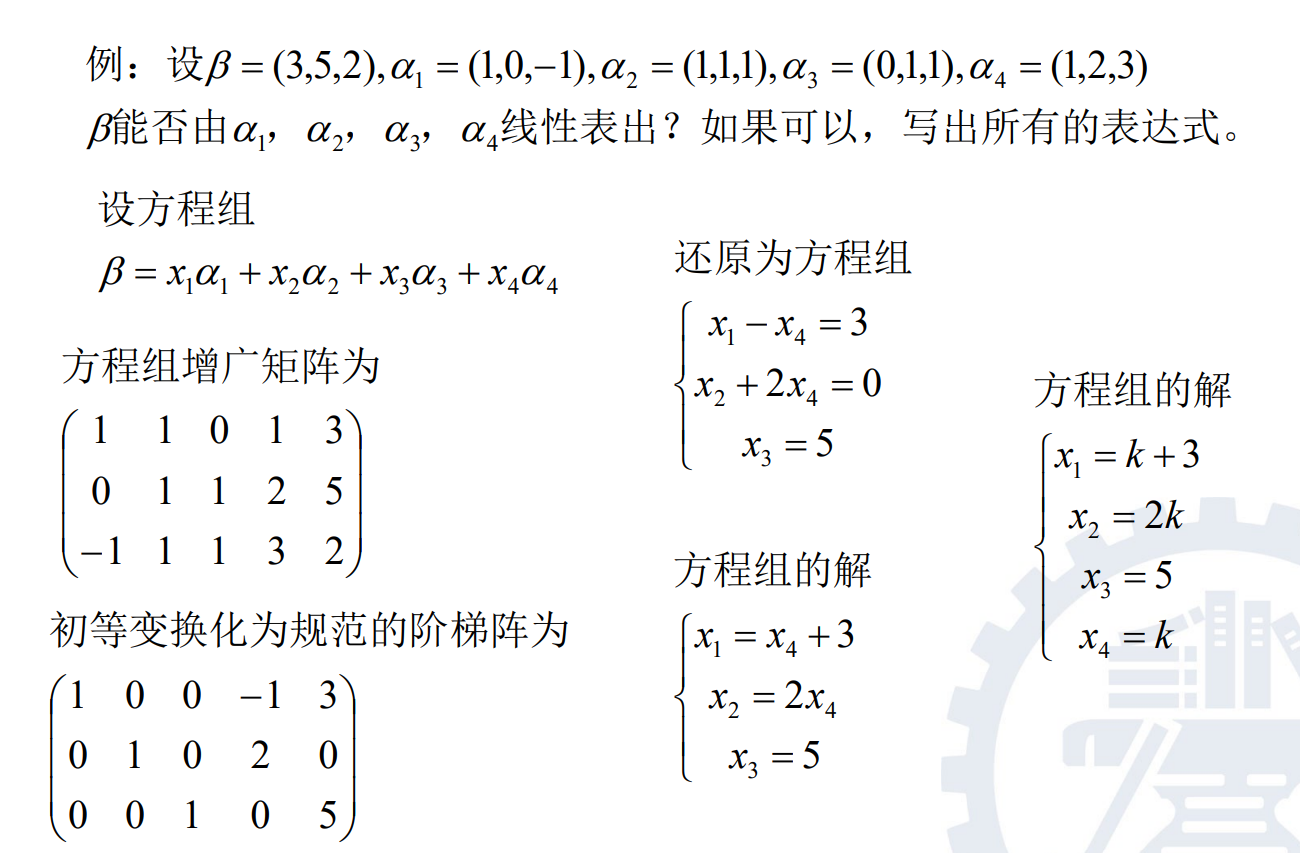
\includegraphics[scale=0.6]{problem3.1.png}
\end{problem}
\begin{property}
    \textbf{传递性}\\
    向量组线性表出具有传递性
    \[\left( \alpha_{1},\alpha_{2},\cdots,\alpha_{s} \right) = \left( \beta_{1},\beta_{2},\cdots,\beta_{t} \right)A\]
    设向量组\(\alpha_{1},\alpha_{2},\cdots,\alpha_{s}\)可由向量组\(\beta_{1},\beta_{2},\cdots,\beta_{t}\)线性表出,
    \[\left( \beta_{1},\beta_{2},\cdots,\beta_{t} \right) = \left( \gamma_{1},\gamma_{2},\cdots,\gamma_{n} \right)B\]
    设向量组\(\alpha_{1},\alpha_{2},\cdots,\alpha_{s}\)可由向量组\(\gamma_{1},\gamma_{2},\cdots,\gamma_{n}\)线性表出,
    \[\left( \alpha_{1},\alpha_{2},\cdots,\alpha_{s} \right) = \left( \beta_{1},\beta_{2},\cdots,\beta_{n} \right)A = \left( \gamma_{1},\gamma_{2},\cdots,\gamma_{n} \right)BA\]
    即向量组\(\alpha_{1},\alpha_{2},\cdots,\alpha_{s}\)可由\(\gamma_{1},\gamma_{2},\cdots,\gamma_{n}\)线性表出
\end{property}
\section{向量组等价}
\begin{definition}
    设有两个向量组\(\alpha_{1},\alpha_{2},\cdots,\alpha_{s}\) 和\(\beta_{1},\beta_{2},\cdots,\beta_{t}\),\(\alpha_{1},\alpha_{2},\cdots,\alpha_{s}\) 可由\(\beta_{1},\beta_{2},\cdots,\beta_{t}\) 线性表出,\(\beta_{1},\beta_{2},\cdots,\beta_{t}\)也可由\(\alpha_{1},\alpha_{2},\cdots,\alpha_{s}\) 线性表出,则称向量组\(\alpha_{1},\alpha_{2},\cdots,\alpha_{s}\)与向量组\(\beta_{1},\beta_{2},\cdots,\beta_{t}\)等价。
    \\ \textbf{向量组等价意味着可以相互表示}
\end{definition}

\begin{property}
    \textbf{向量组的等价关系}
    \begin{enumerate}
        \item 反身性
        \item 对称性
        \item 传递性
    \end{enumerate}
\end{property}

\section{线性相关与线性无关}
\begin{definition}
    设\(\alpha_1,\alpha_2 \dots \alpha_m\)为m个n维度向量,若存在不权威零的数,使
    \[\tag{11.2} k_1\alpha_1 + k_2\alpha_2 + \dots + k_m\alpha_m = 0\]
    则称\(\alpha_1,\alpha_2 \dots \alpha_m\)线性相关
    \\直观上反映:这m个向量中存在多余的向量
    \\否则称他们线性无关。若(11.2)式当且仅当\(k_1=k_2=\cdots=k_m=0\)时成立,则称\(\alpha_1,\alpha_2 \dots \alpha_m\)线性无关。
    \\直观上反映:这m个向量中没有多余的向量
\end{definition}
\begin{property}
    \textbf{线性相关与线性组合的关系} \\
    向量\(\alpha_1,\alpha_2 \dots \alpha_m\)线性相关
    \\ \(\Leftrightarrow\) \(\alpha_1,\alpha_2 \dots \alpha_m\)中至少有一个向量能由其他向量线性表出
    \\(至少有一个多余的)
    \\\textbf{逆否命题:}向量\(\alpha_1,\alpha_2 \dots \alpha_m\)线性无关
    \\ \(\Leftrightarrow\) \(\alpha_1,\alpha_2 \dots \alpha_m\)中任何一个向量都不能由其他向量线性表出
    \\(没有多余的)
\end{property}
\begin{property}
    \textbf{与线性方程组之间的联系} \\
    \(\alpha_1,\alpha_2 \dots \alpha_m\)线性相关(线性无关)
    \\ \(\Leftrightarrow\) 齐次方程组\(k_1\alpha_1 + k_2\alpha_2 + \dots + k_m\alpha_m = 0\)有非零解(仅有唯一零解)
    \\ \textbf{推论1}
    \(\alpha_1,\alpha_2 \dots \alpha_m\)线性相关
    \\ \(\Leftrightarrow\) \(r(A)<m\) (A的秩\(<\)未知数的个数=A的列数=向量个数)
    \\ \textbf{推论2} (结合克拉默法则)
    \\n个n维向量\(\alpha_1,\alpha_2 \dots \alpha_n\)线性相关(无关)
    \\ \(\Leftrightarrow\) \(\rvert \mathbf{A} \rvert = \rvert \alpha_1,\alpha_2 \dots \alpha_n \rvert = 0 (\neq 0)\)
    \\ \textbf{推论3}
    \\ 对于\(\mathbb{R}^n\)中任意m个向量,当\(m > n\)时必线性相关。
\end{property}
\begin{property}
    \textbf{一些重要结论}
    \begin{enumerate}
        \item m个n维向量中,若有含有0向量,则这m个向量线性相关 \\ \textbf{逆否命题:} 若m个n维向量是线性无关的,则这m个向量中没有0向量
        \item m个n维向量中,若有一部分向量线性相关,则这m个向量线性相关
        \item 若m个n维向量是线性无关的,则这m个向量中的任何一部分向量,放在一起,也是线性无关的
        \item 若m个n维向量是线性无关的,那么保持这m个n维向量的分量的相对位置的任何n+k维向量仍然是线性无关的。
        \item 若m个n维向量是线性相关的,那么保持这m个n维向量的分量的相对位置的任何k(≤n)维向量是线性相关的。
    \end{enumerate}
\end{property}

\begin{method}
    \textbf{判断向量组线性相关(线性无关)的方法}
    \\ 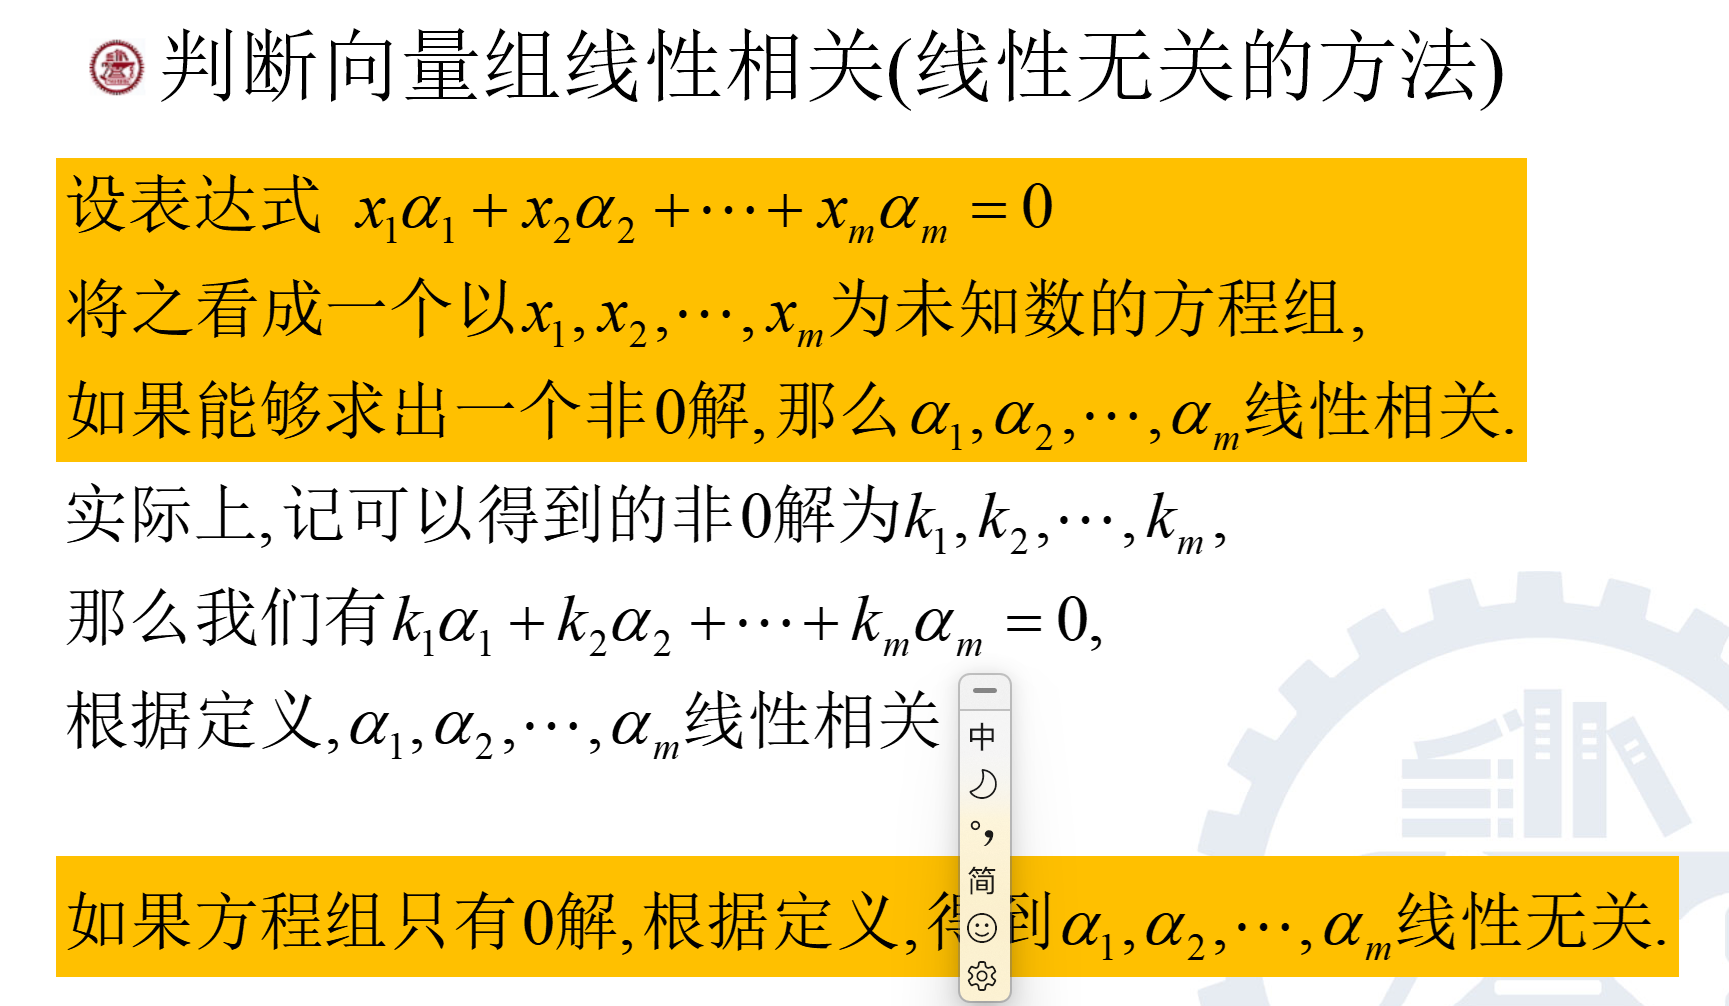
\includegraphics[scale=0.4]{method3.1.png}
\end{method}
\begin{problem}
    \textbf{方程组解法}
    \\ 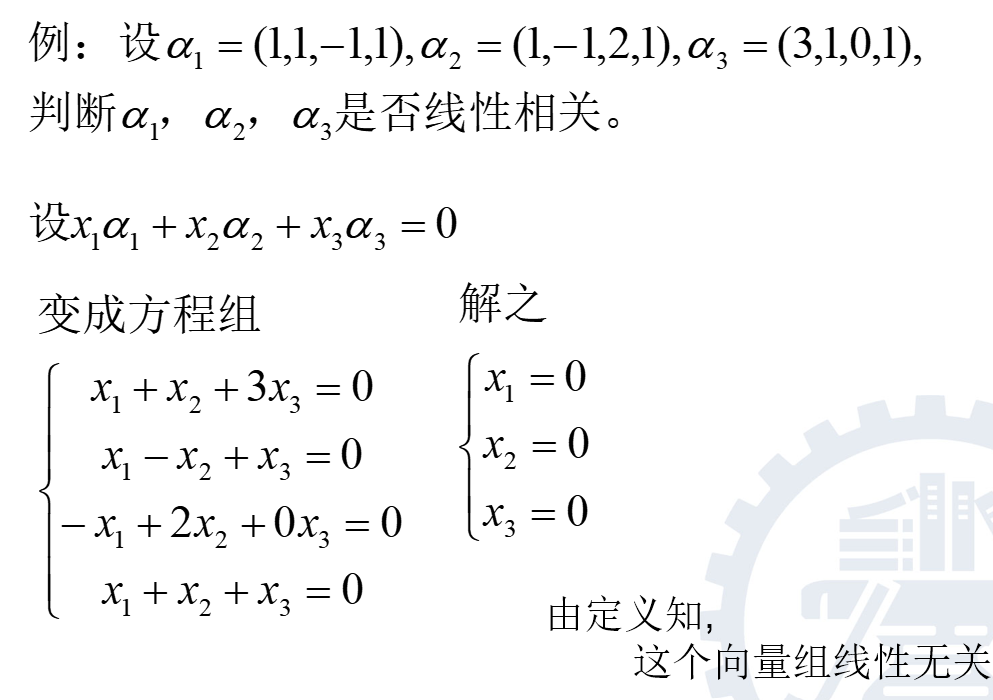
\includegraphics[scale=0.7]{problem3.2.png}
\end{problem}
\begin{problem}
    \textbf{使用克拉默法则,结合行列式}
    \\ 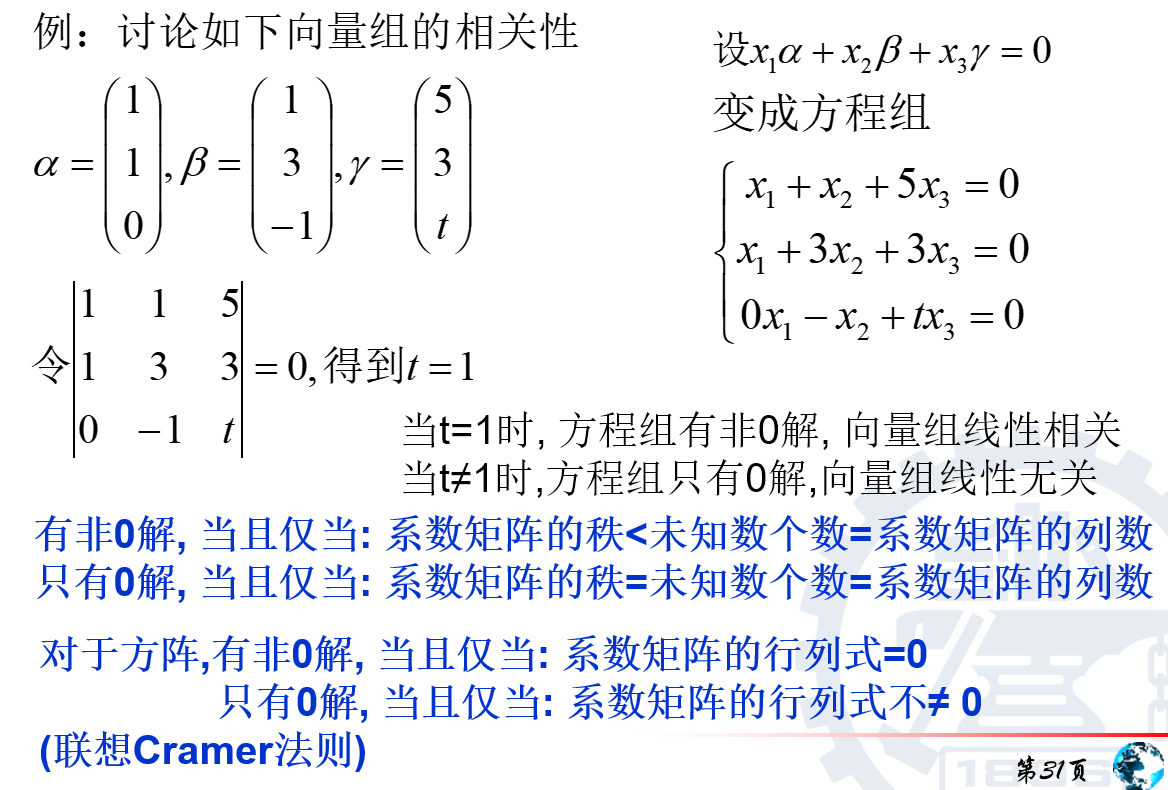
\includegraphics[scale=0.6]{problem3.3.png}
\end{problem}
\begin{property}
    向量\(\alpha_1,\alpha_2 \dots \alpha_m\)线性无关,且\(\alpha_1,\alpha_2 \dots \alpha_m , \beta\)线性相关
    \\ \(\Leftrightarrow\) \(\beta\)可由向量组\(\alpha_1,\alpha_2 \dots \alpha_m\)线性表出,且表出系数唯一。
\end{property}
\end{document}